\section{Iteration 2}
\label{i2}
Der in der ersten Iteration erstellte Prototyp wurde dem Auftraggeber in Form einer Demo gezeigt.
Dabei sind folgenden Rückmeldungen entstanden:

\begin{itemize}
    \item Der Prototyp entspricht den Vorstellungen und erfüllt die definierten Anforderungen.
    \item Die Vorgabe, dass die Benutzerschnittstelle für Mobilgeräte ausgelegt sein soll, fällt weg.
          Sie soll neu für Desktop-Geräte optimiert werden.
    \item Nebst Spannungswerten soll die Applikation auch Leistungs- und \ac{THD} Werte verarbeiten können.
    \item Bisher wurden sämtliche Daten künstlich erstellt.
          Diese sollen um echte Messwerte erweiter werden, welche von Auftraggeber zur Verfügung gestellt werden.
    \item Die Benutzerschnittstelle soll um die Funktion erweitert werden,
          dass eine spezifische Zeitspanne ausgewählt werden kann.
\end{itemize}
In den folgenden Abschnitten wird erläutert,
wie die erforderlichen Anpassungen an den einzelnen Teilen der Applikation vorgenommen wurden.

\subsection{\ac{MQTT} Datenverarbeitung}
\label{i2:mqtt}
Da neu auch die Leistungs- und \ac{THD} Werte der Stromzähler verarbeitet werden sollen, wurde
die \ac{MQTT} Datenverarbeitung angepasst. Der Dataingress erwartet nun, dass nebst
den Spannungen der drei Phasen auch noch die Leistungs- und \ac{THD} Werte mitgeschickt werden.

Um die neuen Daten abspeichern zu können, wurde auch das Datenbankschema entsprechend erweitert.
Das vollständige Datenbankschema wird im Kapitel \ref{rel:db} aufgezeigt.
Auch die bereits vorhandenen Tests mussten so angepasst, dass die neuen Daten
mitgesendet werden.

\begin{figure}[H]
    \centering
    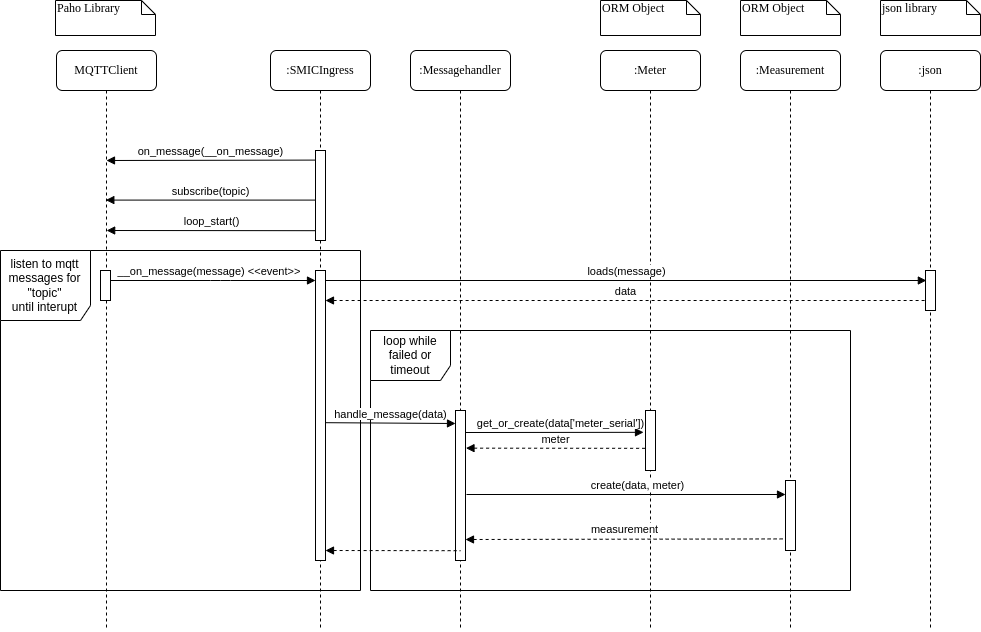
\includegraphics[width=1.0\textwidth]{gfx/dataingress-sequence}
    \caption{
        Implementation von Fehlerbehandlung durch den Messagehandler und einen
        Retry-Loop
    }
    \label{fig:dataingress-sequence}
\end{figure}

Während der Entwicklung zeigte es sich, dass der Dataingress nicht sehr stabil
funktioniert und sporadisch fehlschlägt. Analysen zeigten, dass
die Datenbankverbindung teilweise instabil ist.
Diese Verbindungsprobleme liessen sich auf die verwendete SQLite Datenbank zurückführen.

Es ist davon auszugehen, dass dieses Problem in einer Produktivumgebung mit einem Datenbanksystem wie PostgreSQL
weniger auftreten würde.
Der Code sollte jedoch auf den Fall, dass die Verbindung zur Datenbank nicht hergestellt werden kann, reagieren können,
und sicherstellen, dass keine Daten verloren gehen.
Dazu wurde wie in Abbildung \ref{fig:dataingress-sequence} aufgezeigt
eine Fehlerbehandlung implementiert.
Die empfangenen Daten der Stromzähler
werden nun über einen Messagehandler abgearbeitet.
Schlägt das Schreiben in die Datenbank fehl, versucht es der Messsagehandler nach einem kurzen Zeitintervall erneut.
Nach einer festgelegten Anzahl von Versuchen wird der fehlgeschlagene Schreibversuch in einer Logdatei gespeichert.

\subsection{Fakemeter}
Die im vorherigen Abschnitt erwähnten Anpassungen wurden auch für den Fakemeter umgesetzt.
So konnten die Änderungen am Dataingress direkt getestet werden. 
Der Auftraggeber stellte einen Datensatz von echten Stromzählerdaten
zur Verfügung. Damit diese echten Daten in das System eingelesen werden können,
wurde der Fakemeter noch um einen ``Batch Mode`` erweitert. Das heisst,
er liest das bereitgestellte CSV File mit den Datensätzen ein und sendet die Daten in
gewissen Zeitabständen. Dies soll das Verhalten eines echten Stromzählers
möglichst realitätsnah Simulieren. 

\begin{figure}
    \centering
    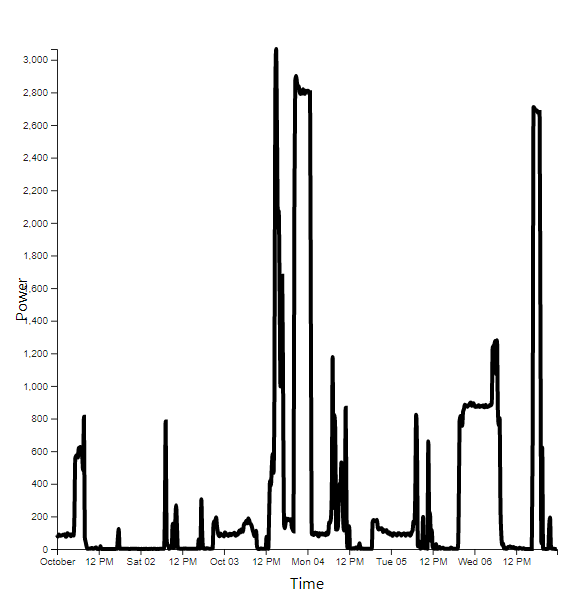
\includegraphics[width=0.5\textwidth]{gfx/markusData}
    \caption{
        Visualisierung der Leistungsdaten, welche vom Auftraggeber bereitgestellt wurden
    }
    \label{fig:markusData}
\end{figure}
Abbildung \ref{fig:markusData} ist ein Screenshot der Applikation und zeigt den
echten Leistungsverlauf eines Haushaltes anfangs Oktober.
Diese Daten wurden mittels Fakemeter übermittelt.
Welche Änderungen an der Benutzerschnittstelle für die Visualisierung nötig waren,
wird in nächsten Abschnitt erläutert.



\subsection{Benutzerschnittstelle}
Um die neuen Anforderungen zur Benutzerschnittstelle zu erfüllen, musste diese neu Entworfen werden.
Das Layout, welches bisher für Mobilgeräte ausgelegt war, konnte sehr einfach für Desktop-Geräte angepasst werden.
In Abbildung \ref{fig:phase2-ui} ist dies zu sehen.
Für die Auswahl eines Zeitintervalls wurden neuen Komponenten oberhalb des Graphen platziert.
Die neuen Leitungs- und \ac{THD} Werte werden in separaten Graphen angezeigt und sind horizontal neben dem bestehenden Graphen angezeigt.
Drei Checkboxen wurden neu hinzugefügt, um die Anzeige der einzelnen Graphen zu steuern.
Ein Dropdown-Menu ermöglicht die Auswahl des Stromzählers, wessen Daten angezeigt werden.
Diese Funktionalität wurde nicht explizit vom Auftraggeber gefordert, war jedoch für das manuelle Testen
und das Demonstrieren der Anwendung sehr praktisch, da so unterschiedliche Daten angezeigt werden können.
\begin{figure}[H]
    \centering
    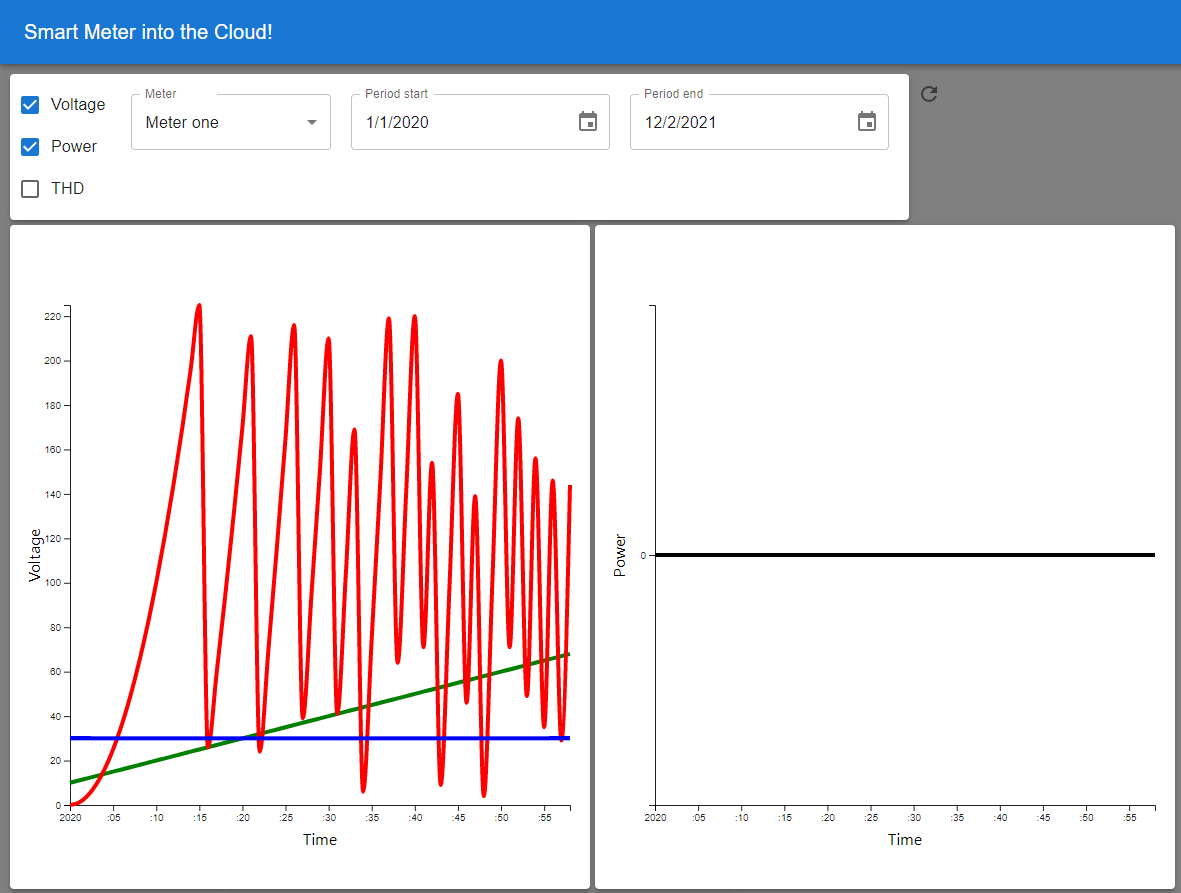
\includegraphics[width=1.0\textwidth]{gfx/phase2}
    \caption{
        Die Benutzerschnittstelle, ausgelegt für Desktop Geräte
    }
    \label{fig:phase2-ui}
\end{figure}
\subsection{\ac{API}}
Im vorherigen Abschnitt wurden neue Filter- und Selektionsfunktionen der Benutzerschnittstelle beschrieben.
Damit diese richtig funktionieren, musste auch die \ac{API} entsprechend erweitert werden.
\begin{verbatim}
    GET /meters
\end{verbatim}
Gibt eine Liste aller in der Datenbank vorhandener Stromzähler zurück, so, dass diese für die Auswahl angezeigt werden.
\begin{verbatim}
    GET /meters/{meter_id}/measurements
\end{verbatim}
Im Body kann neu optional ein Zeitintervall angegeben werden.
Zurückgeben werden dan alle Messungen des Zählers, welche währen des Intervals liegen.



\subsection{Verifikation}

Um die neue Funktionalität des Dataingress zu testen, wurde der in Iteration 1
implementierte Test (Abbildung \ref{fig:test-iteration-1}) um die neue Funktionalität
erweitert.

\subsection{Schwierigkeiten}
Bis auf die im Absatz \ref{i2:mqtt} beschriebenen Instabilitäten der Datenbank konnte
die zweite Iteration ohne grosse Schwierigkeiten durchgeführt werden.
Dies lässt darauf schliessen, dass die erstellten Grundlagen und getroffenen Entscheidungen aus 
der ersten Iteration gut und richtig waren.
